\documentclass[11pt,a4paper]{article}

\usepackage[utf8]{inputenc}
\usepackage[T1]{fontenc}
\usepackage[margin=2.5cm]{geometry}
\usepackage{booktabs}
\usepackage{graphicx}
\usepackage{amsmath}
\usepackage{amssymb}
\usepackage[hidelinks]{hyperref}
\usepackage{enumitem}
\usepackage{caption}
\captionsetup{font=small,labelfont=bf}

\title{A Parcel-Level Crop Classifier for Piura, Peru,\\from Legacy Land-Titling Records and Landsat Imagery\\[0.5em]\large Project status report}
\author{Daniel Ash}
\date{22 July 2026}

\begin{document}
\maketitle

\begin{abstract}
\noindent We are building a supervised crop classifier for farm parcels in Piura, Peru, using
declared crops from legacy land-titling records as labels and Landsat satellite time series as
features. This report documents the project to date: the forensic reconstruction of the source
datasets and their linkage into $(\text{polygon},\ \text{crop},\ \text{year})$ training examples;
the label-cleaning and spatial-splitting pipeline; the current training dataset (49{,}648
parcels, 12 classes) and its known weaknesses; the three-model ladder (LightGBM $\to$ LTAE $\to$
PSE-LTAE) with its input representations and training regime; and the results of the completed
full-scale run of 22 July 2026, in which all three models were trained on the full Landsat
extraction ($4.5$M pixel observations) and all clear the majority-class baseline under spatial
cross-validation. All three models were then retrained and hyperparameter-swept on the revised
12-class label space (30 July 2026); the tuned Lightweight Temporal Attention Encoder now leads
at pooled macro-F1 $0.427$ (versus LightGBM's $0.383$), by rescuing the rare classes that a
gradient-boosted baseline misses. The locked test set remains unspent; the next action is its
single evaluation on the chosen model.
\end{abstract}

\section{Introduction}

The goal is a classifier that, given a farm parcel's polygon boundary and a crop year, predicts
the crop grown from satellite imagery. The training signal is assembled from Peruvian
land-titling (PETT/COFOPRI) archives:
\[
\text{(polygon boundary)} + \text{(declared crop)} + \text{(year)}
\;\longrightarrow\; \text{Landsat time series} \;\longrightarrow\; \text{features} \;\longrightarrow\; \text{label}.
\]
A large share of the work has been \emph{forensic}: the source files are undocumented legacy
datasets whose provenance, keys, and mutual relationships had to be established empirically
before any modelling was possible. The modelling pipeline itself
(labels $\to$ spatial splits $\to$ Google Earth Engine extraction $\to$ feature assembly $\to$
train/evaluate/infer) is now built, unit-tested (47 tests), and verified end-to-end; a
deliberately limited ``medium run'' has been completed to de-risk the full extraction
(Section~\ref{sec:medium}); no model has yet been trained on the full dataset.

\section{Source data}
\label{sec:raw}

\subsection{The raw datasets}

All figures are Piura-only. Two independent crop sources exist --- the PETT/SSET titling
registry (c.~1998--2007) and the 2012 CENAGRO agricultural census --- and they share no parcel
code.

\begin{table}[ht]
\centering\small
\caption{Raw datasets. The starred bridge is the decisive file: it is the only reliable
connection between crop declarations and polygon geometry.}
\begin{tabular}{@{}p{4.6cm}p{6.2cm}rp{3.2cm}@{}}
\toprule
File & What it is & Rows & Key fields \\
\midrule
\texttt{BD SSET(\ldots).xlsx} & PETT land-titling \textbf{crop registry}; one row per
parcel-crop declaration (a panel) & 348{,}076 & \texttt{Codigo SSET}, \texttt{CULTIVO},
\texttt{FECHA}, \texttt{AREA} \\
\texttt{grafica\_tabular\_Piura.dta}~$\star$ & Cadastral \textbf{bridge} carrying both keys &
158{,}427 & \texttt{CodigoSSET} $\leftrightarrow$ \texttt{COD\_PREDIO} \\
\texttt{grafica\_tabular\_catastro\_Piura.dta} & Older, smaller bridge (a strict subset;
superseded) & 109{,}796 & same two keys \\
\texttt{qgis\_stefany/\ldots FINAL.shp} & \textbf{Parcel polygons} (EPSG:32717) & 190{,}098 &
\texttt{COD\_PREDIO} \\
\texttt{qgis\_stefany/PIURA.dta} & Shapefile attribute table; no \texttt{CodigoSSET}, cannot
bridge & 158{,}638 & \texttt{COD\_PREDIO} \\
\texttt{IV\_CENAGRO\_Piura.dta} & 2012 agricultural \textbf{census}; one row per
parcel$\times$crop & 947{,}884 & census codes, farmer name \\
\texttt{IV CENAGRO -- Tabla\_Cultivos.xlsx} & Census crop-code dictionary & 3{,}351 codes &
code $\to$ crop name \\
\texttt{Base\_Cenagro\_PETT\_Piura.dta} & A prior census$\leftrightarrow$PETT merge (comparison
only; no geometry) & 142{,}348 & mixed \\
\bottomrule
\end{tabular}
\end{table}

Two provenance findings mattered. First, despite its filename, the polygon shapefile is a
\textbf{PETT/COFOPRI cadastre}, not census geometry: its census fields are 100\% empty, its PETT
fields are populated, and its embedded lineage shows it was copied from a pre-existing cadastral
layer into the 2012 census geodatabase as a base map. Second, the wider bridge
(\texttt{grafica\_tabular\_Piura.dta}, covering 68.8\% of SSET crop keys) strictly supersedes
the catastro bridge (59.8\%, a subset), recovering $+12{,}842$ crop records and $+8{,}392$
polygons.

\subsection{The linkage}

The training set is built from \textbf{Chain A}, which uses real keys only:
\[
\text{BD SSET (crop, year)} \xrightarrow{\texttt{CodigoSSET}}
\text{bridge} \xrightarrow{\texttt{COD\_PREDIO}}
\text{polygons (geometry)}.
\]
This yields \textbf{116{,}599 crop records over 66{,}363 distinct polygons}. A second chain
links the 2012 census to PETT parcels by normalised farmer name (the census has no shared code);
it is reliable for the person and crop but agrees with a reference merge on the \emph{exact}
parcel only $\sim$43\% of the time, so it is held in reserve as a weak second time point and is
not used for training.

\subsection{Fundamental limitations of the labels}
\label{sec:limits}

These properties of the source data are load-bearing for every downstream choice:

\begin{itemize}[leftmargin=1.5em]
\item \textbf{The year is a titling date, not a growing season.} Registration dates cluster on
batch/stub values (a single stub date accounts for $\sim$35\% of rows). We therefore model the
full 12-month phenological profile of the labelled year and accept a label--season mismatch as
an irreducible accuracy ceiling (locked decision A1).
\item \textbf{One crop-year per parcel.} Only 1 of 66{,}363 polygons has crops declared in more
than one distinct year: the data is a single c.~1998--99 snapshot, not a panel. There is no
temporal train/test axis --- only a spatial one. About 80\% of labels fall in 1998--99.
\item \textbf{Only Landsat covers the label years.} The bulk of crop years pre-date Sentinel-2
(2015+) by 15+ years; Landsat~5/7 at 30\,m resolution is the only year-matched sensor.
\item \textbf{Parcels are tiny relative to the sensor.} Median parcel area is 0.42\,ha
$\approx$ 4--5 Landsat pixels; $\sim$75\% of parcels contain no pure interior pixel after a
one-pixel erosion, so edge-mixed pixels are the norm.
\item \textbf{Crops grow in single-crop blocks.} $\sim$86\% of adjacent parcels share a crop
(vs.\ $\sim$46\% under random placement). Any random train/test split leaks a parcel's
spectral twin (its neighbour) across the split; spatial blocking is mandatory.
\item \textbf{Intercropping is real} ($\sim$16\% of linked polygons carry more than one crop,
e.g.\ \emph{CAFE Y PLATANO}) and requires an explicit policy.
\end{itemize}

\section{Data processing}
\label{sec:processing}

\subsection{Crop-label normalisation}

The raw \texttt{CULTIVO} field is free text: 9{,}394 distinct raw strings with typos, accents,
plural/singular variants, regional synonyms, and multi-crop cells separated by every delimiter
imaginable (including percentage weightings such as \emph{CAFE 50\%--PLATANO 50\%}). A curated
normaliser maps each cell to a \emph{list} of $(\text{crop},\ \text{category})$ pairs, where the
category is one of \texttt{crop} / \texttt{pasture} / \texttt{fallow} / \texttt{land\_prep} /
\texttt{unspecified}. Nothing is dropped at this stage --- non-crops are only flagged --- and
genuinely distinct crops (e.g.\ bean varieties) are never merged. The 9{,}394 raw labels
compress to $\sim$1{,}647 canonical tokens; every mapping decision is recorded in an audit CSV,
and the tricky cases are pinned by unit tests.

The scripted pipeline then joins SSET $\to$ bridge $\to$ polygons, cleans implausible years and
non-positive areas, dissolves duplicate geometries, and aggregates to \textbf{one row per
polygon}: 66{,}352 polygons with a normalised crop list, category list, modal year, and area.

\subsection{Label policy (from crop lists to a single class)}

The modelling label is derived per parcel: a single named crop becomes its class; a single
pasture or fallow token becomes a \texttt{PASTURE} / \texttt{FALLOW} land-cover class;
\texttt{land\_prep} and \texttt{unspecified} tokens are dropped (not observable crops).
Multi-crop parcels are looked up in a configurable \emph{merge map} of 24 domain-decided
entries (extended 22 July 2026): coffee-shade systems (\emph{CAFE + PLATANO / NARANJA /
GUABO / pasture / sugar cane}) $\to$ \texttt{CAFE}; cacao systems $\to$ \texttt{CACAO};
orchard--annual mixes $\to$ the perennial (visible year-round, e.g.\ \emph{MAIZ+MANGO} $\to$
\texttt{MANGO}); lime--mango orchards $\to$ a new \texttt{MIXED\_ORCHARD} class;
annual--annual mixes $\to$ the declared main crop (e.g.\ \emph{FRIJOL+MAIZ} $\to$
\texttt{MAIZ}); and crop + fallow/land-preparation tokens $\to$ the crop. The map keeps
4{,}936 intercropped parcels; unmatched intercrops are excluded. There is \emph{no}
\texttt{other} bucket: crops with fewer than 300 eligible parcels are dropped (1{,}733
parcels; this removed \texttt{CACAO}, an intended merge target that reached only
$\sim$100 parcels). Two further class-surgery steps were added on 22 July 2026 after the
first full-scale results: \texttt{GIRASOL} was dropped outright (355 parcels; it sits in
only 4 spatial regions and every model scored $\approx$0 on it), and the perennial-orchard
classes \texttt{MANGO}, \texttt{LIMON}, and \texttt{MIXED\_ORCHARD} were collapsed into a
single \texttt{MANGO\_LIMON} class (2{,}298 parcels; the merged class spans 119 regions,
far healthier spatial support than any component). Hard gates exclude parcels with area
outside $[0.09, 50]$\,ha (sub-pixel or implausibly large) or a year outside $[1990, 2020]$.

\begin{table}[ht]
\centering\small
\caption{Parcels excluded by the label policy.}
\begin{tabular}{@{}lr@{}}
\toprule
Exclusion reason & Parcels \\
\midrule
Area outside 0.09--50\,ha & 9{,}041 \\
Multi-crop, not in merge map & 4{,}577 \\
Rare crop ($<$300 parcels) dropped & 1{,}787 \\
Dropped category (land-prep / unspecified) & 999 \\
Missing year & 0 \\
\bottomrule
\end{tabular}
\end{table}

\subsection{Spatial split}
\label{sec:split}

Because of the block structure of cropping (Section~\ref{sec:limits}), the split is spatial
throughout. Parcels are assigned to a 1\,km block grid and a 5\,km region grid (metric CRS,
EPSG:32717). An autocorrelation audit measures pairwise crop agreement against distance:
agreement is 0.75 under 100\,m and is still 0.37 at 4--5\,km against a 0.24 random baseline ---
i.e.\ the decorrelation range exceeds 5\,km.

Design consequences:
\begin{itemize}[leftmargin=1.5em]
\item \textbf{Held-out sets are contiguous 5\,km regions}, not scattered blocks. A buffered
dead-zone around held-out data costs training parcels in proportion to held-out
\emph{perimeter}; with scattered 1\,km test blocks the buffer excluded 69\% of all parcels,
whereas contiguous test regions cost only $\sim$8{,}500 buffer exclusions.
\item \textbf{A locked test set} of whole regions ($\approx$15--19\% of parcels; currently
9{,}689 parcels in 59 regions) is touched exactly once, at the end of the project. Every class
is forced into test where possible.
\item \textbf{Five cross-validation folds} are formed over the remaining regions with
stratified group $k$-fold; per-fold buffer flags keep each fold's training set at least
1.5\,km away from its validation regions.
\item \textbf{Residual leakage is a known, accepted limitation}: the 1.5\,km buffer is smaller
than the $>$5\,km decorrelation range, so scores are slightly optimistic near region borders.
A wider buffer was considered and deliberately rejected (it trades training data for purity);
the decision will be revisited if the locked-test score falls well below cross-validation.
\end{itemize}

\section{The dataset before training}
\label{sec:final}

The label policy and split produce \texttt{modeling\_parcels.parquet}: \textbf{49{,}648 parcels
in 12 classes} (40{,}503 train/validation, 9{,}145 locked test in 58 regions), spread over
2{,}076 populated 1\,km blocks in 246 regions. The full Landsat extraction already covers every
parcel, and 48{,}106 (96.9\%) pass the $n\geq4$ coverage gate.

\begin{table}[ht]
\centering\small
\caption{Class distribution (49{,}648 parcels; label policy of 22 July 2026, v3). ARROZ = rice,
MAIZ = maize, ALGODON = cotton, TRIGO = wheat, CA\~NA DE AZUCAR = sugar cane, FRIJOL = bean,
PLATANO = banana, ZARANDAJA = hyacinth bean. FALLOW/PASTURE are land-cover classes;
MANGO\_LIMON is the merged mango/lime/mixed-orchard perennial class.}
\begin{tabular}{@{}lrr@{}}
\toprule
Class & Parcels & Share \\
\midrule
ARROZ & 21{,}564 & 43.4\% \\
FALLOW & 8{,}734 & 17.6\% \\
MAIZ & 5{,}809 & 11.7\% \\
ALGODON & 3{,}235 & 6.5\% \\
CAFE & 2{,}859 & 5.8\% \\
MANGO\_LIMON & 2{,}298 & 4.6\% \\
PASTURE & 2{,}210 & 4.5\% \\
TRIGO & 1{,}162 & 2.3\% \\
FRIJOL & 617 & 1.2\% \\
PLATANO & 493 & 1.0\% \\
CA\~NA DE AZUCAR & 364 & 0.7\% \\
ZARANDAJA & 303 & 0.6\% \\
\bottomrule
\end{tabular}
\end{table}

\subsection{Known problems, by year, crop, and parcel}
\label{sec:problems}

\paragraph{Years.} 39\% of parcels (18{,}861) carry year 1998, which is Landsat-5-only (no
Landsat~7 until 1999) and coincides with the strong 1997--98 El Ni\~no cloud season. A GEE
availability audit found a parcel-weighted average of only $\sim$5.5 valid (clear) months per
parcel-year, with gaps that are \emph{contiguous} rather than scattered: 62\% of parcels have a
$\geq$3-month missing block. This is why the pipeline never interpolates onto a dense time grid
--- interpolation would fabricate exactly the unobserved phenology the classifier needs. The
medium run (Section~\ref{sec:medium}) has since quantified the 1998 problem precisely: parcels
are \emph{not lost} (the coverage gate passes 95.4\% of them) but their signal is thin (median
5 clear observations vs.\ 8 in 1999).

\paragraph{Crops.} The set is severely imbalanced (ARROZ 43\%, top two classes 61\%), so
macro-F1 --- not accuracy --- is the primary metric, and losses are class-weighted. Some
classes have thin \emph{spatial} support regardless of parcel count: ZARANDAJA has only 5
locked-test parcels and CAFE's test parcels sit in 4 regions, so their test numbers will be
anecdotal (GIRASOL, the worst case, was dropped from the vocabulary after scoring
$\approx$0 for every model; MANGO/LIMON's support problem was solved by merging them into
MANGO\_LIMON). The 24-entry merge map keeps 4{,}936 intercropped parcels; the 4{,}577
multi-crop parcels outside it remain excluded, and further map extensions are still the
cheapest way to grow the training set.

\paragraph{Parcels.} The median parcel (0.42\,ha) spans only $\sim$4--5 Landsat pixels and
usually has no pure interior pixel, so all spectral summaries are edge-contaminated; this
motivates the pixel-set encoder rung of the model ladder. Sub-pixel parcels ($<$0.09\,ha) are
excluded by the area gate. Parcels whose satellite coverage was never measured, or that fail
the quality gate below, are excluded from training and \emph{abstained} at inference rather
than silently filled.

\section{Satellite features}
\label{sec:features}

\paragraph{Extraction (Google Earth Engine).} Landsat Collection-2 Level-2 surface reflectance,
with missions chosen by crop year (L5 through 2013, L7 from 1999, L8 from 2013) and bands
harmonised to \{Blue, Green, Red, NIR, SWIR1, SWIR2\}. Clouds, shadows, dilated cloud, cirrus
(QA\_PIXEL) and saturated pixels (QA\_RADSAT) are masked. Extraction is two-stage:
\begin{enumerate}[leftmargin=1.5em]
\item \textbf{Coverage pass}: per parcel-year, count clear acquisitions (\texttt{n\_valid\_obs})
and the longest run of empty months (\texttt{max\_gap}). The \textbf{abstain gate}
\texttt{n\_valid\_obs} $\geq 4$ decides which parcels are worth extracting; the same fixed gate
is shared by all models and by inference, keeping metrics comparable.
\item \textbf{Pixel pass, gate survivors only}: every clear pixel observation (raw reflectance,
pixel location, day of year, mission) is exported once into a raw store. Both model
representations are re-assembled from this store offline, so GEE is never hit twice.
\end{enumerate}
Extraction is chunked, resumable, and content-addressed; transient GEE errors are retried with
exponential backoff, and oversized computations are split automatically.

\paragraph{Assembly.} From the raw store, with 11 channels per observation (6 bands + NDVI,
EVI, NDWI, NDMI, BSI), and \emph{no binning or interpolation}:
\begin{itemize}[leftmargin=1.5em]
\item a \textbf{tabular feature row} per parcel (141 columns): per-channel
median/mean/std/min/max/quartiles/amplitude, a linear slope, and an order-1 \textbf{harmonic
fit} (mean, cosine, sine terms --- encoding phenology peak timing without a time grid; NaN when
under 4 observations), plus statics (area, latitude, \texttt{n\_valid\_obs}, \texttt{max\_gap},
L7 fraction);
\item a \textbf{per-date sequence tensor} $X \in \mathbb{R}^{N\times 64\times 11}$ of
parcel-median spectra at real irregular dates, with day-of-year positions and a validity mask;
\item a \textbf{pixel-set tensor} $X \in \mathbb{R}^{N\times 64\times 8\times 11}$ keeping the
8 most-observed 30\,m pixels per parcel per date, with a pixel mask.
\end{itemize}
NDVI trajectories from the pilot extraction are agronomically sound: rice and cotton show
mid-year cycles; coffee and banana stay high year-round.

\section{Models}
\label{sec:models}

Three models form a controlled ladder --- each rung adds exactly one capability, so a win
identifies \emph{which} capability earned it. All share one interface
(\texttt{fit} / \texttt{predict\_proba} / \texttt{save} / \texttt{load}) and output a
probability vector over the class vocabulary (currently 12 classes); the predicted class is
the arg-max, subject to
abstention (below).

\begin{table}[ht]
\centering\small
\caption{The model ladder.}
\begin{tabular}{@{}llp{4.5cm}p{4.5cm}@{}}
\toprule
\# & Model & Input & Adds over previous \\
\midrule
1 & \textbf{LightGBM} & 141-column whole-year summary + harmonic row (NaN-native) & the
baseline to beat \\
2 & \textbf{LTAE} & per-date median sequences $[64,11]$ + DOY + mask & temporal attention over
irregular dates \\
3 & \textbf{PSE-LTAE} & pixel sets $[64,8,11]$ + DOY + masks & a learned pixel-distribution
encoder \\
\bottomrule
\end{tabular}
\end{table}

\begin{enumerate}[leftmargin=1.5em]
\item \textbf{LightGBM} trains on the tabular row with class weights and native missing-value
handling. It is expected to be a strong baseline and runs on CPU.
\item \textbf{LTAE} (Lightweight Temporal Attention Encoder; Garnot \& Landrieu) applies masked
attention over the per-date median vectors with sinusoidal day-of-year encoding. Attention, not
recurrence, is the right backbone because the observation gaps are long and contiguous: it
weights the few real acquisitions directly instead of propagating recurrent state across a
4--5-month void.
\item \textbf{PSE-LTAE} replaces the per-date median with a \emph{pixel-set encoder} (masked
mean+std pooling over the clear pixels of each date) feeding the \emph{same} LTAE temporal
core, so the rung-2$\to$3 delta isolates the value of learning the pixel distribution --- the
principled version of hand-picked percentiles, and the state of the art for small,
variable-pixel parcels.
\end{enumerate}

Alternatives requiring a dense, NaN-free temporal grid (TempCNN, MiniRocket, InceptionTime)
were rejected on principle: they force the interpolation this data forbids. The Torch models
run unmodified on Apple-Silicon MPS and CUDA (automatic device selection with CPU fallback);
channel normalisation statistics are fit on the training subset only and stored inside each
saved model.

\subsection{Training regime and evaluation protocol}
\label{sec:regime}

Training proceeds as: \textbf{5-fold spatial cross-validation} (each fold's training set
excludes its validation regions' 1.5\,km buffer) $\to$ \textbf{final refit} on all
train/validation parcels minus the test buffer $\to$ \textbf{one} evaluation on the locked test
set, spent only on the final chosen model and never used for tuning. Hyperparameter search
(Optuna) optimises mean CV macro-F1 only. The neural models use AdamW, class-weighted
cross-entropy, and early stopping on validation macro-F1; per the project's milestone gating,
the LTAE/PSE-LTAE work proceeds only if LightGBM beats the majority-class baseline under
spatial CV.

Evaluation reports macro-F1 (primary), weighted F1, balanced accuracy, Cohen's $\kappa$, the
majority-class baseline, a per-class table, a row-normalised confusion matrix, a reliability
curve with Brier score, and macro-F1 stratified by parcel area, observation count, gap length,
and year. Inference over any parcel table \textbf{abstains} rather than guessing --- reasons:
coverage never measured; failed the $n\geq4$ gate; no features; or top probability below a
confidence threshold $\tau$ --- and coverage (share of parcels scored) is always reported
alongside accuracy so models with different abstention are not conflated.

\section{Results of the medium de-risking run (21 July 2026)}
\label{sec:medium}

Before committing to the full extraction, a deliberately limited run extracted 20 chunks each
of years 1998 and 1999 (both stages), assembled features, and trained LightGBM under the full
spatial-CV protocol (the locked test set was not touched). Its purpose was to measure the
feared 1998 attrition, per-year gate pass rates, and the full-run cost --- not to produce a
competitive model. (Note: this run predates the 22 July label revision, so it was trained on
the previous 48{,}289-parcel label space, which still contained an \texttt{other} bucket and
lacked \texttt{MIXED\_ORCHARD}; its coverage and cost findings are unaffected.)

\paragraph{Coverage and the 1998 question.} The gate is \emph{not} the problem:

\begin{table}[ht]
\centering\small
\caption{Coverage-gate results by year (medium run; ``measured'' = parcels with a completed
coverage pass).}
\begin{tabular}{@{}lrrrr@{}}
\toprule
Year & Measured & Pass ($n\geq4$) & Pass rate & Median clear obs \\
\midrule
1998 & 8{,}000 & 7{,}628 & 95.4\% & 5 \\
1999 & 8{,}139 & 7{,}823 & 96.1\% & 8 \\
2000 & 117 & 112 & 95.7\% & 13 \\
\bottomrule
\end{tabular}
\end{table}

\noindent The L5-only 1998 cohort passes the gate at the same rate as 1999, but its signal is
thin: median 5 clear observations versus 8, and roughly $4\times$ fewer pixel observations per
parcel-chunk. In the CV predictions, 1998 parcels scored accuracy 0.13 versus 0.47 for 1999
(confounded with fold geography and the small 1998 sample --- to be re-checked at full scale).
Conclusion: 1998 will contribute \emph{weak}, not \emph{missing}, signal.

\paragraph{Cost.} Eighty chunks completed in 6\,min\,44\,s ($\approx$7\,s/chunk, both stages,
zero errors or retries), projecting the full extraction at \textbf{$\approx$2.5 hours}
(coverage remainder $\approx$9\,min; $\approx$1{,}150 pixel chunks $\approx$2.4\,h).

\paragraph{Model.} With 1{,}921 feature-bearing parcels ($\approx$4\% of the eventual training
data), pooled-CV LightGBM achieved macro-F1 $0.102$ (per-fold $0.108 \pm 0.045$), accuracy
$0.372$ versus a majority-class baseline of $0.393$, and $\kappa = 0.13$. The model does
\textbf{not yet beat the majority baseline} --- the expected outcome at this scale, not a
failure: per-fold training sets of 563--1{,}267 parcels cannot support 15 classes. Real signal
is nonetheless present: FALLOW reaches F1 $0.58$, ARROZ $0.34$, ALGODON $0.15$, while all rare
classes score zero. The stratified breakdown behaves as designed: accuracy is $0.54$ for
parcels with \texttt{max\_gap} $\leq 2$ months versus $0.08$ beyond 4 months, confirming that
the coverage diagnostics capture feature quality.

\section{Results of the full run (22 July 2026)}
\label{sec:full}

The full pipeline then ran end to end without error: coverage measurement for all parcels
(96.9\% pass the $n\geq4$ gate), raw-pixel extraction for every survivor (1{,}219 chunks,
\textbf{4.53 million pixel observations over 47{,}851 parcels}, $\approx$2.5\,h of GEE time,
zero failed chunks), feature assembly, and training of all three models under the buffered
spatial-CV protocol. These runs used the 15-class label space current at the time (before the
GIRASOL/MANGO\_LIMON revision of Section~\ref{sec:processing}); the locked test set was not
touched.

\begin{table}[ht]
\centering\small
\caption{Full-run results. Fold column: spatial-CV macro-F1 mean $\pm$ s.d.\ over the five
folds. Remaining columns: pooled over all 38{,}535 cross-validation predictions.
Baselines: majority-class accuracy 0.424, majority macro-F1 0.040.}
\begin{tabular}{@{}lccccc@{}}
\toprule
Model & CV macro-F1 & Pooled macro-F1 & Balanced acc. & Accuracy & Cohen's $\kappa$ \\
\midrule
LightGBM & $0.311 \pm 0.034$ & 0.307 & 0.310 & \textbf{0.545} & 0.414 \\
LTAE & $0.347 \pm 0.018$ & \textbf{0.358} & \textbf{0.408} & 0.527 & 0.404 \\
PSE-LTAE & $0.348 \pm 0.009$ & \textbf{0.358} & 0.400 & 0.523 & 0.401 \\
\bottomrule
\end{tabular}
\end{table}

\noindent Key findings:
\begin{itemize}[leftmargin=1.5em]
\item \textbf{Milestone 3 is passed}: every model clears the majority baseline (LightGBM
accuracy 0.545 vs.\ 0.424; $\kappa = 0.41$), which green-lit the attention models.
\item \textbf{The attention models earn their $+0.05$ macro-F1 on rare classes.} ZARANDAJA
goes from F1 0.01 (LightGBM) to 0.55 (PSE-LTAE); TRIGO from 0.43 to 0.65; CA\~NA DE AZUCAR
from 0.10 to 0.18. LightGBM keeps a small edge on the majority classes (hence its higher
plain accuracy) --- the expected trade under class weighting.
\item \textbf{Strong classes are strong for every model}: ARROZ $\approx$0.75, CAFE
$\approx$0.68--0.72, FALLOW $\approx$0.50, PASTURE $\approx$0.48 --- agronomically sensible
(flooding cycle, evergreen canopy).
\item \textbf{PSE-LTAE $\approx$ LTAE} (0.358 vs.\ 0.358): the pixel-set encoder does not yet
beat a per-date median on these tiny parcels, though it halves the fold-to-fold variance.
\item Training cost is low: LTAE $\approx$16\,min and PSE-LTAE $\approx$35\,min on an
M3 MacBook Air (MPS), so hyperparameter sweeps are affordable.
\end{itemize}

Artifacts: comparison figures in \texttt{runs/model\_comparison\_20260722/} (per-fold
macro-F1, pooled metrics, per-class F1 by model); per-run bundles (row-normalised confusion
matrix, reliability curve, per-class and stratified CSVs, per-fold training curves for the
neural models) in \texttt{runs/lightgbm\_20260722\_162635}, \texttt{runs/ltae\_20260722\_163303},
and \texttt{runs/psetae\_20260722\_164933}.

\section{Results on the revised 12-class label space (30 July 2026)}
\label{sec:12c}

All three models were then retrained on the revised label space (GIRASOL dropped,
MANGO/LIMON/MIXED\_ORCHARD merged into MANGO\_LIMON; 49{,}648 parcels, 12 classes). Because a
label change only re-joins the cached Landsat features at training time, no new GEE extraction
or feature assembly was needed. Each model was then hyperparameter-tuned with a 30-trial Optuna
search (objective: mean 3-fold spatial-CV macro-F1, never touching the test set), and the best
configuration refit under the full five-fold protocol. Both attention sweeps selected
$d_{\text{model}}=128$; LTAE preferred heavier dropout (0.45) and a gentler learning rate
($4.5\times10^{-4}$).

\begin{table}[ht]
\centering\small
\caption{Tuned 12-class results (current state of the art). Fold column: spatial-CV macro-F1
mean $\pm$ s.d.\ over five folds; remaining columns pooled over all 38{,}682 cross-validation
predictions. Baseline: majority-class accuracy 0.425.}
\begin{tabular}{@{}lccccc@{}}
\toprule
Model (tuned) & CV macro-F1 & Pooled macro-F1 & Accuracy & Cohen's $\kappa$ & Run \\
\midrule
LightGBM  & $0.379 \pm 0.049$ & 0.383 & \textbf{0.576} & \textbf{0.445} & \texttt{lightgbm\_12c\_tuned} \\
\textbf{LTAE} & $0.409 \pm 0.033$ & \textbf{0.427} & 0.559 & 0.437 & \texttt{ltae\_12c\_tuned} \\
PSE-LTAE  & $0.409 \pm 0.044$ & 0.421 & 0.540 & 0.421 & \texttt{psetae\_12c\_tuned} \\
\bottomrule
\end{tabular}
\end{table}

\noindent Key findings:
\begin{itemize}[leftmargin=1.5em]
\item \textbf{The label revision was worth more than tuning.} Dropping the unlearnable GIRASOL
and merging the lime/mango orchards lifted the best macro-F1 from 0.358 (15-class) to
$\approx$0.42; the Optuna sweeps added only a further $\approx$0.01--0.02.
\item \textbf{The attention advantage holds and widens the rare-class gap.} ZARANDAJA rises
from F1 0.09 (LightGBM) to 0.46--0.48; TRIGO from 0.48 to 0.67. LightGBM retains the accuracy
edge and is better on MAIZ (0.27 vs.\ 0.23) and PASTURE (0.51 vs.\ 0.45).
\item \textbf{PSE-LTAE still does not beat LTAE} --- the pixel-set encoder does not earn its
extra cost on these $\approx$0.5\,ha parcels. Plain LTAE is the leading candidate for the test
evaluation.
\item \textbf{Fold~0 remains everyone's hardest region} (macro-F1 $\approx$0.29 for LightGBM,
0.36--0.37 for the neural models) with a normal class/year mix --- genuine regional difficulty,
and the honest error bar.
\end{itemize}

Artifacts: comparison figures in \texttt{runs/model\_comparison\_12c/} (Figures~\ref{fig:pooled}
and \ref{fig:perclass}); sweep histories in \texttt{runs/sweep\_ltae\_20260730*} and
\texttt{runs/sweep\_psetae\_20260730*}; per-run evaluation bundles under each
\texttt{runs/\{ltae,psetae\}\_12c*} directory.

\begin{figure}[ht]
\centering
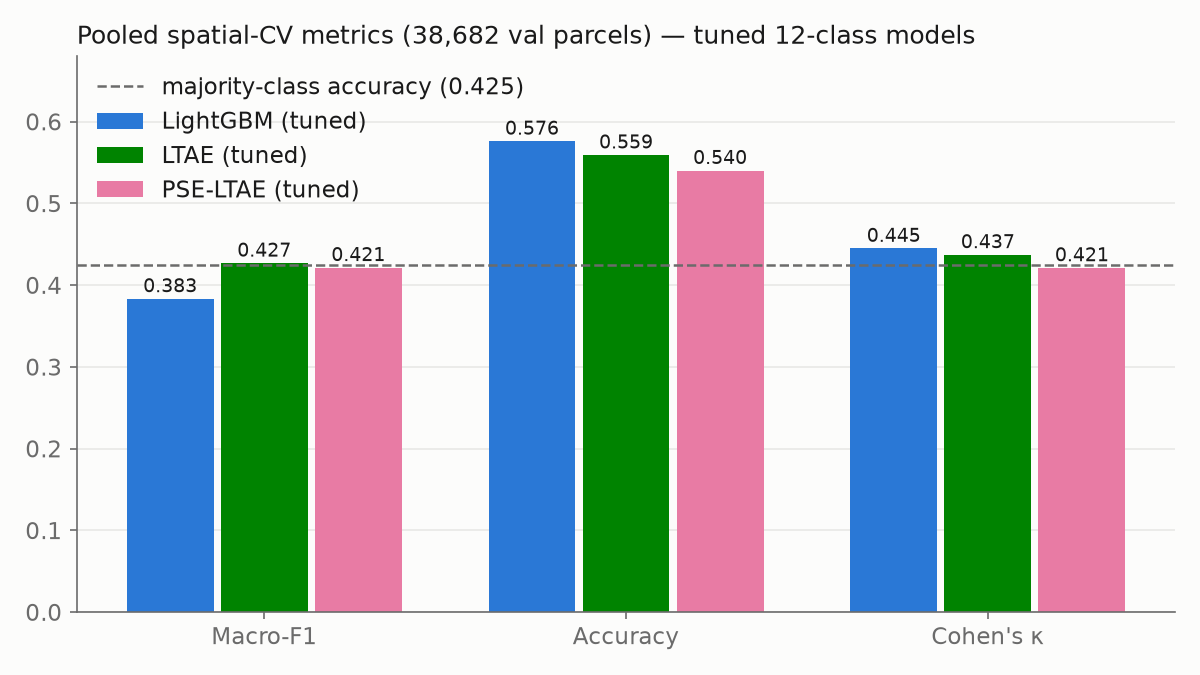
\includegraphics[width=0.82\textwidth]{figures/pooled_cv_metrics.png}
\caption{Pooled spatial-CV metrics for the three tuned 12-class models. All clear the
majority-class accuracy baseline (dashed). LTAE leads on macro-F1; LightGBM leads on plain
accuracy and $\kappa$.}
\label{fig:pooled}
\end{figure}

\begin{figure}[ht]
\centering
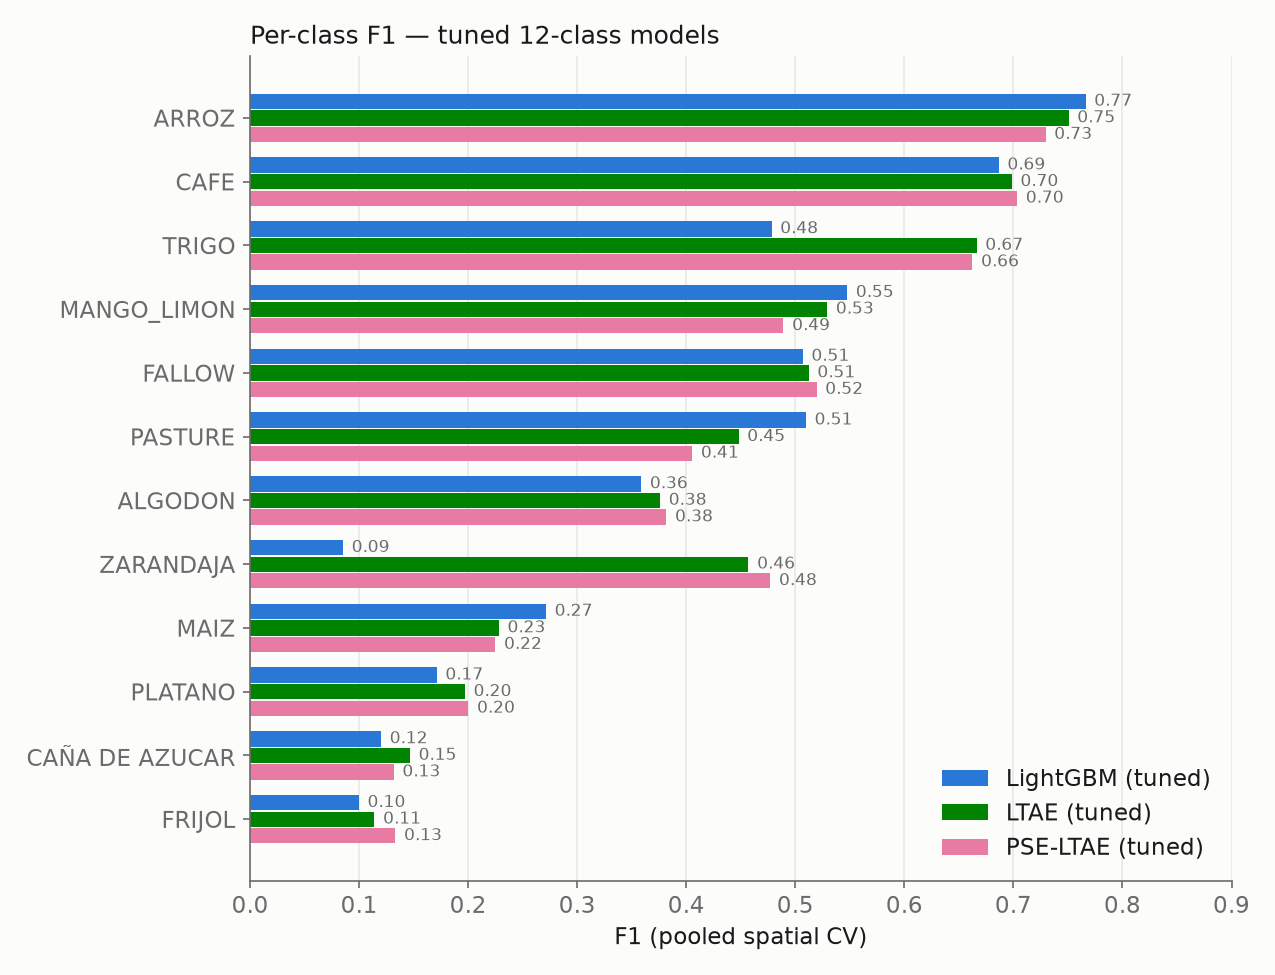
\includegraphics[width=0.82\textwidth]{figures/per_class_f1.png}
\caption{Per-class F1 (pooled spatial CV). The attention models' advantage is concentrated in
the rare classes (ZARANDAJA, TRIGO); the head classes (ARROZ, CAFE) are strong for all three.}
\label{fig:perclass}
\end{figure}

\section{Next steps and outstanding choices}
\label{sec:next}

\paragraph{Immediate.}
\begin{enumerate}[leftmargin=1.5em]
\item \textbf{Retrain all three models on the revised 12-class label space} ---
\emph{done} (Section~\ref{sec:12c}).
\item \textbf{Optuna sweeps on the model family} --- \emph{done} for all three models
(Section~\ref{sec:12c}). Remaining: the \texttt{max\_gap} training-filter ablation, and
optionally temperature scaling of the neural probabilities (pooled Brier $\approx$0.22) before
relying on confidence-based abstention.
\item Spend the locked test set \emph{once} on the chosen model (tuned LTAE), reporting
coverage alongside accuracy.
\end{enumerate}

\paragraph{Outstanding choices.}
\begin{itemize}[leftmargin=1.5em]
\item \textbf{Intercrop merge map}: extended to 24 entries on 22 July 2026 (4{,}936 parcels
kept); 4{,}577 multi-crop parcels remain excluded, and a multi-label head stays deferred.
\texttt{CACAO} was an intended merge target but fell below the 300-parcel class minimum and is
dropped --- recoverable by lowering \texttt{min\_class\_parcels} or adding more cacao combos.
\item \textbf{Rare-class policy}: GIRASOL is resolved (dropped); ZARANDAJA stays in the
vocabulary --- the attention models can learn it (CV F1 $\approx$0.5) --- but its 5-parcel
locked-test support means its test number must be reported as ``insufficient spatial
support''.
\item \textbf{Buffer width}: keep 1.5\,km (accepting slight optimism) unless locked-test
scores fall well below CV, in which case widen and retrain.
\item \textbf{\texttt{max\_gap} training filter}: an ablatable, perennial-aware exclusion of
badly-gapped annual parcels from training (default off); the medium-run stratification
(accuracy $0.54 \to 0.08$ across gap bins) suggests this ablation is worth running.
\item \textbf{Untuned defaults}: sequence length $T_{\max}=64$, pixel-set size $P=8$, harmonic
minimum of 4 observations, and all model hyperparameters await the Optuna sweeps on real data.
\item \textbf{1998 handling}: if full-scale results confirm the weak 1998 cohort, options are a
year covariate (already a feature), per-cohort reporting, or down-weighting 1998 labels ---
exclusion is a last resort given the cohort is 39\% of the data.
\item \textbf{The 2012 census link} (name-based, parcel-uncertain) remains available as a weak
second time point or an external validation source, but is out of scope for the current runs.
\end{itemize}

\end{document}
